% !TEX root = ../../../I4PRJ, Grp3 - Rapport.tex
\chapter{Grafisk Design}
I dette afsnit beskrives det grafiske design af brugergrænsefladen. Det grafiske design skal afspejle de respektive views funktionalitet. Først udarbejdes et konceptuelt design. GUI views designes ved at analyserer og diskuterer user stories for systemet. Resultatet af analysen er et håndtegnet design med tilhørende noter fra diskussionerne. Analyseresultatet dannede grundstenene for GUI folkenes arbejde. Designet blev dermed ensartet for de forskellige platforme. Det fælles udarbejdede design har mindsket en muligt senere kommende bureaukratisk proces, da alle udviklere ved at målet er nået, når GUI svarer til design. 

\section{Konceptuel Design}
Først udarbejdes et konceptuelt design. Det konceptuelle design udarbejdes ved analyse og diskussion af user stories, som eksempel er user story omhandlende login behandlet og kan ses på figuren nedenfor:

\begin{figure}
	\centering
	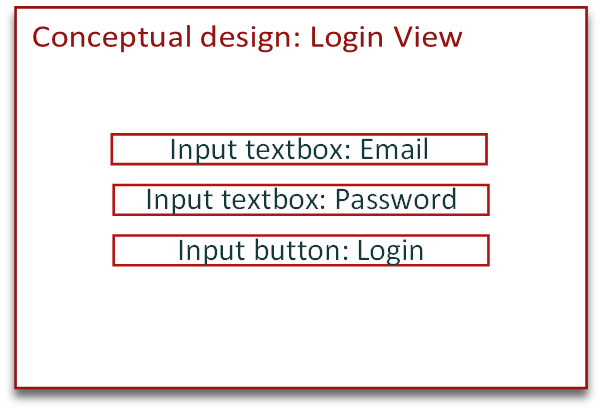
\includegraphics[width=\linewidth]{figs/design/concuptuel_design_loginview}
	\caption{Domænemodel for systemet}
	\label{fig:domainmodel}
\end{figure}

De konceptuelle design udvikles

De forskellige platformes GUI minder i så høj grad om hinanden, at hvert view og hvilke user stories de implementerer kun vil blive beskrevet for en platform. 